\documentclass[12pt]{article}

\usepackage[utf8]{inputenc}
\usepackage{amsmath,amsthm,amsfonts,amssymb,amscd}
\usepackage{multirow,booktabs}
\usepackage[table]{xcolor}
\usepackage{fullpage}
\usepackage{lastpage}
\usepackage{enumitem}
\usepackage{fancyhdr}
\usepackage{mathrsfs}
\usepackage{wrapfig}
\usepackage{setspace}
\usepackage{calc}
\usepackage{multicol}
\usepackage{cancel}

\usepackage{graphicx}
%%\usepackage{caption}
%%\usepackage{subcaption}


\usepackage{listings}
\usepackage{matlab-prettifier}
\usepackage[framed,numbered,autolinebreaks,useliterate]{mcode}

\usepackage[margin=3cm]{geometry}
\newlength{\tabcont}
\setlength{\parindent}{0.0in}
\setlength{\parskip}{0.05in}
\usepackage{empheq}
\usepackage{framed}
\usepackage[most]{tcolorbox}
\usepackage{xcolor}
\colorlet{shadecolor}{orange!15}
\parindent 0in
\parskip 12pt
\geometry{margin=1in, headsep=0.25in}
\usepackage{float}
\usepackage{graphicx}
\usepackage{hyperref}


\newtheorem{thm}{Theorem}
\theoremstyle{theorem}
\newtheorem{reg}{Rule}
\newtheorem{exe}{Exercise}
\newtheorem{rem}{Remark}
\newtheorem{cor}{Corollary}
\newtheorem{exa}{Example}

\usepackage{natbib}
\bibliographystyle{abbrv}

\usepackage{times}

%\usepackage[compact]{titlesec}
\usepackage{titlesec}
\titlespacing*{\section}{0pt}{*-2}{*-1}

\def\a{\alpha}
\def\b{\beta}
\def\de{\delta}
\def\De{\Delta}
\def\ga{\gamma}
\def\Si{\Sigma}
\def\si{\sigma}
\def\ep{\varepsilon}
\def\ze{\zeta}
\def\om{\omega}
\def\leq{\leqslant}
\def\rar{\rightarrow}
\def\Rar{\Rightarrow}
\def\td{\Leftrightarrow}
\def\R{\hro{R}}
\def\C{\hro{C}}
\def\hro{\mathbb}
\def\bbI{\hro{I}}
\def\N{\hro{N}}
\def\Z{\hro{Z}}

\def\tE{\tilde{E}}
\def\hE{\hat{E}}
\def\tA{\tilde{A}}
\def\tT{\tilde{T}}
\def\hA{\hat{A}}
\def\hD{\hat{D}}
\def\bA{\breve{A}}
\def\tB{\tilde{B}}
\def\hB{\hat{B}}
\def\tC{\tilde{C}}
\def\tN{\tilde{N}}
\def\hN{\hat{N}}
\def\tk{\tilde{k}}
\def\tX{\tilde{X}}
\def\hX{\hat{X}}
\def\bX{\breve{X}}
\def\tM{\tilde{M}}
\def\tm{\tilde{m}}
\def\bM{\breve{M}}
\def\hM{\hat{M}}
\def\bm{\breve{m}}
\def\tH{\tilde{H}}
\def\tF{\tilde{F}}
\def\tG{\tilde{G}}
\def\hG{\hat{G}}
\def\tK{\tilde{K}}
\def\tx{\tilde{x}}
\def\tf{\tilde{f}}
\def\hf{\hat{f}}
\def\brf{\breve{f}}
\def\baf{\bar{f}}
\def\tg{\tilde{g}}
\def\hg{\hat{g}}
\def\lb{\lambda}
\def\cP{{\cal P}}
\def\cQ{{\cal Q}}
\def\fr{\frac}
\def\frQ{\mathfrak{Q}}

\def\cU{{\cal U}}
\def\cV{{\cal V}}
\def\cH{{\cal H}}
\def\tcU{{\tilde{\cal U}}}
\def\cZ{{\cal Z}}

\def\hxi{\widehat{\xi}}
\def\hp{\hat{q}}

\def\ddt{\fr{\mathrm{d}}{\mathrm{d}t}}
\def\dtau{\Delta_{\tau}}
\def\tnu{\tilde{\nu}}
\def\tU{\tilde{U}}

\def\tcQ{{\tilde{\cal Q}}}
\def\tcP{{\tilde{\cal P}}}
\def\hcP{\widehat{\cP}}
\def\hcQ{\widehat{\cQ}}
\def\cE{\mathcal{E}}
\def\cA{\mathcal{A}}
\def\cD{\mathcal{D}}
\def\hcE{\hat{\cE}}
\def\hcA{\hat{\cA}}
\def\hcD{\hat{\cD}}
\def\vphi{\varphi}

\newcommand{\n}[1]{\left\lVert#1\right\rVert}

\newcommand{\m}[1]{
	\begin{bmatrix}
		#1
	\end{bmatrix}
}

\renewcommand{\pm}[1]{
	\begin{matrix}
		#1
	\end{matrix}
}

\def\ES{
	\begin{bmatrix}
		J^E  & 0        & 0       & 0 \\
		0       & N^E_{2} & 0       & 0 \\
		0       & 0        & N^E_{3}& 0 \\
		0       & 0        & 0       & N^E_{4} 
	\end{bmatrix}
}

\def\AS{
	\begin{bmatrix}
		A_{1}  & 0       & 0          &  0        \\
		0           & J^A  & 0          & 0      \\
		0           &   0                & N^A_{3}      & 0      \\
		0           &   0                & 0                    & N^A_{4}      
	\end{bmatrix}
}
\def\BS{
	\begin{bmatrix}
		B_{1}  & 0       & 0        & 0 \\
		0          & B_{2}       & 0        & 0 \\
		0          & 0                  & J^B  & 0  \\
		0          & 0                 &   0                & N^B_{4}  \\ 
	\end{bmatrix}
}

\def\be{\begin{equation}}
\def\ee{\end{equation}}         

\newcommand{\ben}{\begin{eqnarray}}
\newcommand{\een}{\end{eqnarray}}

\newcommand{\bens}{\begin{eqnarray*}}
\newcommand{\eens}{\end{eqnarray*}}

\def\bc{\begin{cases}}
\def\ec{\end{cases}}

\newcommand{\bsq}{\begin{subequations}}
\newcommand{\esq}{\end{subequations}}

\newcommand{\eproof}{\space
	{\ \vbox{\hrule\hbox{\vrule height1.3ex\hskip0.8ex\vrule}\hrule}}\\[0.2cm]}

\begin{document}
% \setcounter{section}{8} This is assumed that count from Section 9
\thispagestyle{empty}

\begin{center}
	{\LARGE \bf Chapter 4 Interpolation Schemes}\\[.2cm]
	{\large Numerical Analysis 1. Winter Semester 2018-19}
\end{center}

\section{Polynomial interpolations}

\subsection{Langrange interpolation}

\begin{figure}[h!]
\centering
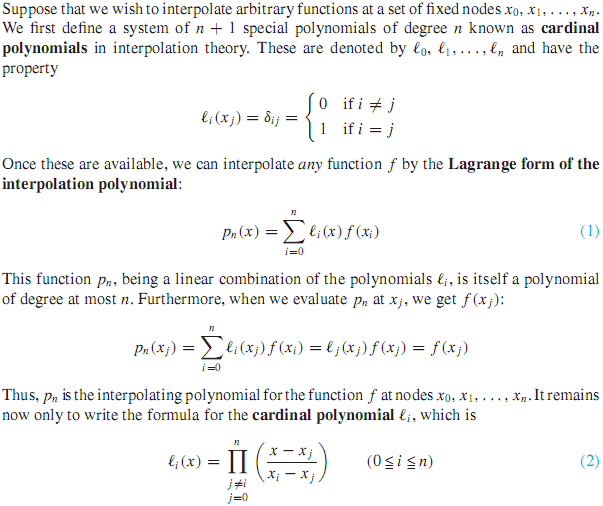
\includegraphics[scale = 0.9]{Figures/12}
\label{Lagrange}
\end{figure}

\textbf{Notice} Example with first and second order Lagrange polynomial. 

\subsection{Newton interpolation}

\textbf{Observation:} The Lagrange formula is well-suited for many theoretical uses of interpolation, but it is less desirable when actually computing the value of an interpolating polynomial. As an example, knowing $P_2(x)$ does not lead to a less expensive way to evaluate $P_3(x)$, 
at least not in a simple manner. For this reason, we introduce an alternative and more easily calculable formulation for the interpolation polynomials $P_1(x)$, $P_2(x), \dots, P_n(x)$. \\
%
\textbf{Idea: Newton interpolation polynomial}
%
\begin{equation*}
 p(x) = c_0 + c_1 (x-x_0) + c_2 (x-x_0) (x-x_1) + \dots + c_{n} (x-x_0)(x-x_1)...(x-x_n).
\end{equation*}
%
\begin{shaded}
It can not be overemphasized that the Newton and Lagrange forms are just two different derivations for precisely the same polynomial.
The Newton form has the advantage of easy extensibility to accommodate additional data points. 
\end{shaded}

\begin{exa} Using the Newton algorithm, find the interpolating polynomial of least degree for this table:
\begin{center}
\begin{tabular}[6]{l|l|l|l|l|l}
x & 0 & 1 & -1 & 2 & -2 \\ \hline 
y & -5 & -3 & -15 & 39 & -9
\end{tabular}
\end{center}
The solution is $p(x)= -5 + 2x - 4x(x-1)+ 8x(x-1)(x+1) + 3x(x-1)(x+1)(x-2)$. 
\end{exa}

\subsection{Error in polynomial interpolation}

See \cite{AtkH03}, page 138-140. For the behavior of the error, see page 142-143 in the same book.

\begin{figure}[h!]
	\centering
	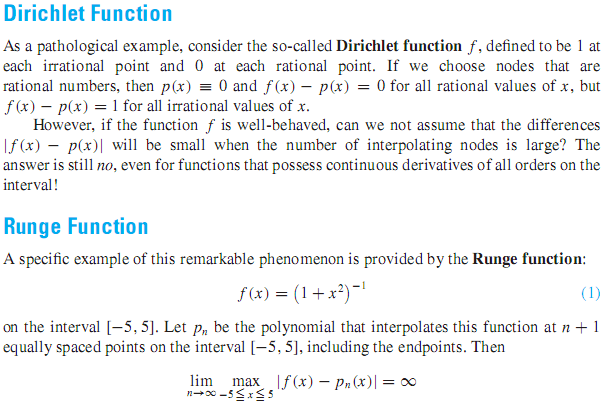
\includegraphics[scale = 0.9]{Figures/15}
	\caption{Page 154, \cite{CheK07}}
\end{figure}


\begin{figure}[h!]
	\centering
	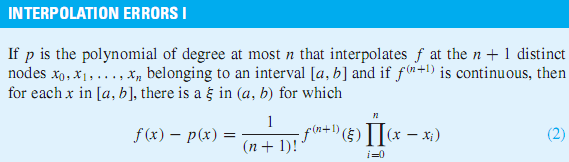
\includegraphics[scale = 0.9]{Figures/16}
\end{figure}

\begin{figure}[h!]
	\centering
	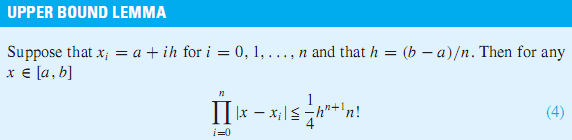
\includegraphics[scale = 0.9]{Figures/17}
\end{figure}

\begin{figure}[!h]
	\centering
	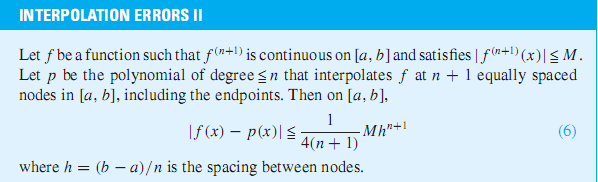
\includegraphics[scale = 0.9]{Figures/18}
\end{figure}


\section{Divided difference and its applications}

We introduce a discrete version of the derivative of a function 

\begin{shaded}
\begin{tabular}[2]{ll}
$f[x_0,x_1] = \cfrac{f(x_1)-f(x_0)}{x_1 - x_0}$ & first-order divided difference, \\[.3cm]
$f[x_0,x_1,x_2] = \cfrac{f[x_1,x_2]-f[x_0,x_1]}{x_2 - x_0}$ & second-order divided difference, \\[.3cm]
$f[x_0,x_1,x_2,x_3] = \cfrac{f[x_1,x_2,x_3]-f[x_0,x_1,x_2]}{x_3 - x_0}$ & third-order divided difference,\\
\end{tabular}

and so on ...
%
\[ 
f[x_0,x_1,\dots,x_n] = \cfrac{f[x_1,\dots,x_n]-f[x_0,\dots,x_{n-1}]}{x_n - x_0}
\]
%
\end{shaded}

\begin{figure}[!h]
	\centering
	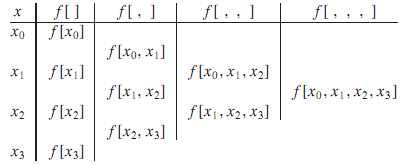
\includegraphics[scale = 0.8]{Figures/25}
	\caption{Scheme to compute divided difference \cite{CheK07}}
\end{figure}

\begin{exa} Computing the divided difference from the following table
	\begin{center}
		\begin{tabular}[5]{l|l|l|l|l}
			x & 1 & 3/2 & 0 & 2  \\ \hline 
			y & 3 & 13/4 & 3 & 5/3
		\end{tabular}
	\end{center}
The solution is $p(x)= 3 + 1/2 (x-1) + 1/3 (x-1)(x-3/2) -2(x-1)(x-3/2)x$. 
\end{exa}

\begin{shaded} Newton interpolation polynomial can be computed based on divided difference
%
\bens 
P_n(x) = f(x_0)+f[x_0,x_1](x-x_0) &+&f[x_0,x_1,x_2](x-x_0)(x-x_1)+ \dots + \\ 
                                        &+& f[x_0,x_1,\dots,x_n](x-x_0)\cdots(x-x_{n-1}).
\eens
%	
Evaluating $P_n(x)$ using nested multiplication
	%
	\[ P_n(x) =  D_0 + (x-x_0) [D_1 + (x-x_1) [D_2 + \dots + (x-x_{n-2}) [D_{n-l} + (x - x_{n-1})D_n] ...
	\]
	%
\end{shaded}
%
\begin{rem} Properties of divided difference. \\
i) Divided difference does not depend on the permutation order of the points $x_0,\dots,x_n$. \\
ii) The divided difference can be extended to the case where some or all of the node points $x_i$ are coincident, provided that $f(x)$ is sufficiently differentiable. 
\end{rem}

\begin{figure}[!h]
	\centering
	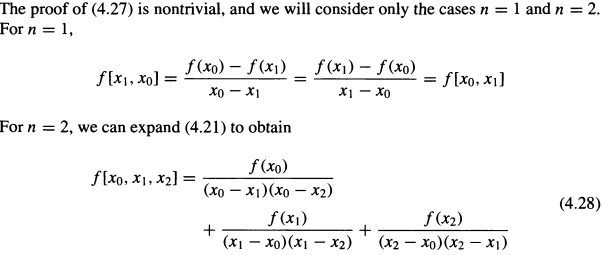
\includegraphics[scale = 0.8]{Figures/24}
	\caption{Proof of property i)}
\end{figure}

\begin{figure}[h!]
	\centering
	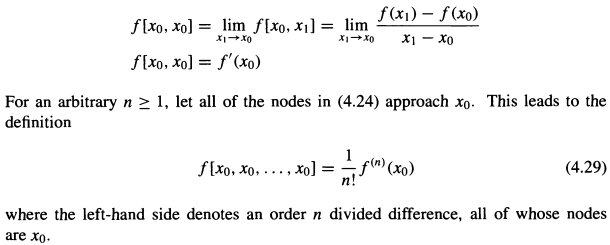
\includegraphics[scale = 0.8]{Figures/26}
	\caption{Property ii) is continued here.}
\end{figure}

\begin{figure}[h!]
	\centering
	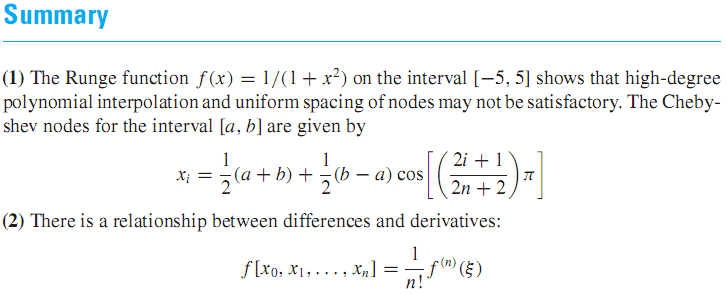
\includegraphics[scale = 0.85]{Figures/19}
\end{figure}

\begin{figure}[h!]
	\centering
	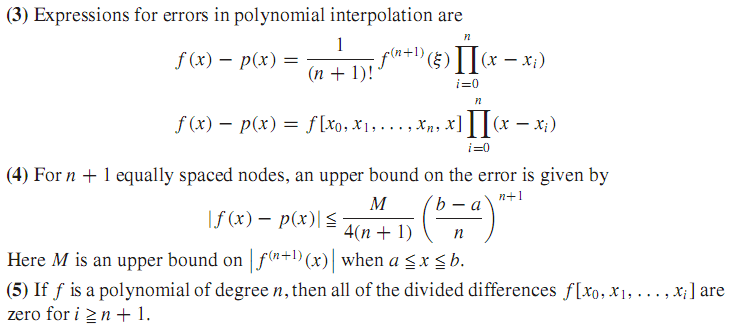
\includegraphics[scale = 0.85]{Figures/20}
\end{figure}

\subsection{Matlab code for Newton interpolation using divided difference}

\begin{shaded}
	\lstinputlisting[language=Matlab]{Matlab_codes/div_diff.m}
	\vskip -.5cm
	\lstinputlisting[language=Matlab]{Matlab_codes/newton_interp.m}
\end{shaded}

Newton’s divided-difference formula can be expressed in a simplified form when the
nodes are arranged consecutively with equal spacing $h=x_{i+1}-x_i$. Using binomial-coefficient notation, we can express $P_n(x)$ compactly as
%
\[  
P_n(x) = P_n(x_0 + sh) = f [x_0] + \sum_{k=1}^{s} \binom{s}{k} k!h^k \ f[x_0, x_1, . . . , x_k].
\]
%
Then, we can have forward Newton difference, backward Newton difference, center difference (Stirling) formulae. See \cite{BurF10}, p.129-133 for further details.

\section{Neville interpolation}

Another method of obtaining a polynomial interpolant from a given table of values was given by Neville. It builds the polynomial in steps, just as the Newton algorithm does. The constituent polynomials have interpolating properties of their own. We start with constant polynomials $P_i(x) = f(x_i)$. 
Selecting two nodes $x_i$ and $x_j$ with $i>j$, we define recursively
\begin{figure}[h!]
	\centering
	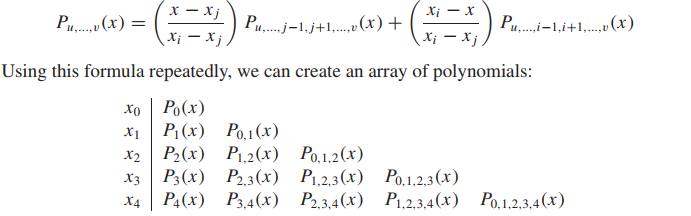
\includegraphics[scale = 0.85]{Figures/27}
\end{figure}
Here, each successive polynomial can be determined from two adjacent polynomials in the previous column. 
%
\begin{thm}
$P_{u,...,v}$ is exactly the Lagrange polynomial that interpolates $f$ at the points $x_u, x_{u+1},\dots,x_v$.
\end{thm}
%
We can simplify the notation by letting
%
\[ S_{i,j}(x) = P_{i-j,i-j+1,\dots,i}(x)  \]
%
where $S_{ij}(x)$ for $i \geq j$ denotes the interpolating polynomial of degree $j$ on the $j + 1$ nodes $x_{i-j}, \dots, x_{i-1}, x_i$. 
Next we can rewrite the recurrence relation above as
%
\begin{shaded}
\[ S_{i,j}(x) = \cfrac{x-x_{i-j}}{x_i-x_{i-j}} S_{i,j-1}(x) -  \cfrac{x-x_i}{x_i-x_{i-j}} S_{i-1,j-1}(x) \mbox{ for all } i\geq j\]
\end{shaded}
%
then $S_{n,n}$ is exactly the value $P_{0,1,\dots,n}(x)$. The Matlab implementation of this, however, has a small modification, since the indices begin from $0$. 
\begin{shaded}
	\lstinputlisting[language=Matlab]{Matlab_codes/neville_interp.m}
\end{shaded}

\section{What have not been covered?}

\begin{shaded}
In this script we have not consider the following topics.
\begin{enumerate}
 \item[i)] Spline interpolation, see \cite{AtkH03}, Section 4.3 and \cite{CheK07}, Chapter 9. 
 \item[ii)] Hermit interpolation, see \cite{BurF10}, Section 3.4. 
 \item[iii)] Estimating derivatives and Extrapolation, see \cite{CheK07}, Section 4.2.
 \item[iv)] Bivariate interpolation, see \cite{CheK07}, Section 4.2.
\end{enumerate}
\end{shaded}

\newpage

\nocite{*}

\bibliography{GTS_reference} 

\end{document}